%\documentclass[10pt,dvipsnames]{beamer}
\documentclass[10pt,svgnames]{beamer}

\definecolor{links}{HTML}{2A1B81}
\hypersetup{colorlinks,linkcolor=,urlcolor=links}

\usetheme[numbering=fraction]{metropolis}
\metroset{block=fill}
%\setmonofont{Ubuntu Mono}

\usepackage{appendixnumberbeamer}

\usepackage{booktabs,empheq,bbold,bm}
\usepackage[scale=2]{ccicons}

\usepackage{pgfplots}
\usepackage{tikz}
\usetikzlibrary{math, positioning}

\usepgfplotslibrary{dateplot}

\usepackage{xspace}
\newcommand{\themename}{\textbf{\textsc{metropolis}}\xspace}

% for python listings; inspired by https://gist.github.com/YidongQIN/a10dd4f72381362aff4257e7a5541d86 
\usepackage{listings}
\usepackage{color}
\definecolor{darkred}{rgb}{0.6,0.0,0.0}
\definecolor{darkgreen}{rgb}{0,0.50,0}
\definecolor{lightblue}{rgb}{0.0,0.42,0.91}
\definecolor{orange}{rgb}{0.99,0.48,0.13}
\definecolor{grass}{rgb}{0.18,0.80,0.18}
\definecolor{pink}{rgb}{0.97,0.15,0.45}
\lstdefinelanguage{PythonPlus}[]{Python}{
  morekeywords=[1]{,as,assert,nonlocal,with,yield,self,True,False,None,} % Python builtin
  morekeywords=[2]{,__init__,__add__,__mul__,__div__,__sub__,__call__,__getitem__,__setitem__,__eq__,__ne__,__nonzero__,__rmul__,__radd__,__repr__,__str__,__get__,__truediv__,__pow__,__name__,__future__,__all__,}, % magic methods
  morekeywords=[3]{,object,type,isinstance,copy,deepcopy,zip,enumerate,reversed,list,set,len,dict,tuple,range,xrange,append,execfile,real,imag,reduce,str,repr,}, % common functions
  morekeywords=[4]{,Exception,NameError,IndexError,SyntaxError,TypeError,ValueError,OverflowError,ZeroDivisionError,}, % errors
  morekeywords=[5]{,ode,fsolve,sqrt,exp,sin,cos,arctan,arctan2,arccos,pi, array,norm,solve,dot,arange,isscalar,max,sum,flatten,shape,reshape,find,any,all,abs,plot,linspace,legend,quad,polyval,polyfit,hstack,concatenate,vstack,column_stack,empty,zeros,ones,rand,vander,grid,pcolor,eig,eigs,eigvals,svd,qr,tan,det,logspace,roll,min,mean,cumsum,cumprod,diff,vectorize,lstsq,cla,eye,xlabel,ylabel,squeeze,}, % numpy / math
}
\lstdefinestyle{colorEX}{
  basicstyle=\ttfamily\small,
  backgroundcolor=\color{white},
  commentstyle=\color{darkgreen}\slshape,
  keywordstyle=\color{blue}\bfseries\itshape,
  keywordstyle=[2]\color{blue}\bfseries,
  keywordstyle=[3]\color{grass},
  keywordstyle=[4]\color{red},
  keywordstyle=[5]\color{orange},
  stringstyle=\color{darkred},
  emphstyle=\color{pink}\underbar,
}
\lstset{style=colorEX,
        basewidth = {.49em}}

\newtheorem*{defn}{definition}
\newtheorem*{thm}{theorem}
\newtheorem*{question}{question}
\newtheorem*{conjecture}{conjecture}
\newtheorem*{proposition}{proposition}

\newtheorem*{cproblem}{continuum problem}
\newtheorem*{feproblem}{finite element problem}

\newcommand{\bg}{\mathbf{g}}
\newcommand{\bn}{\mathbf{n}}
\newcommand{\bq}{\mathbf{q}}
\newcommand{\bu}{\mathbf{u}}

\newcommand{\bU}{\mathbf{U}}

\newcommand{\bzero}{\bm{0}}

\newcommand{\cH}{\mathcal{H}}
\newcommand{\cK}{\mathcal{K}}
\newcommand{\cV}{\mathcal{V}}
\newcommand{\cX}{\mathcal{X}}

\newcommand{\RR}{\mathbb{R}}

\newcommand{\nn}{\mathrm{n}}
\newcommand{\pp}{\mathrm{p}}
\newcommand{\qq}{\mathrm{q}}
\newcommand{\rr}{\mathrm{r}}

\newcommand{\eps}{\epsilon}
\newcommand{\grad}{\nabla}
\newcommand{\Div}{\nabla\cdot}

\newcommand{\rhoi}{\rho_{\text{i}}}
\newcommand{\snew}{s^{\text{new}}}

\newcommand{\sdoi}[1]{\,{\scriptsize \href{https://doi.org/#1}{doi:#1}}}
\newcommand{\surl}[2]{\,{\scriptsize \href{#1}{#2}}}

\newcommand{\comm}[1]{{\footnotesize \hfill \emph{#1}}}
\newcommand{\where}[1]{\text{\footnotesize #1}}
\newcommand{\viewin}[1]{{\footnotesize \emph{this view appears in} #1}}

\renewcommand*{\thefootnote}{\fnsymbol{footnote}}

\newcommand{\aler}[1]{{\color{FireBrick} #1}}


\title{Surface elevation errors \\ in finite element Stokes models \\ for glacier evolution}

\date{Numerical Analysis Seminar, KTH \& SU (September 2025)}

\author{Ed Bueler, University of Alaska Fairbanks}

\titlegraphic{\vspace{-1cm}\par\hspace{-1cm}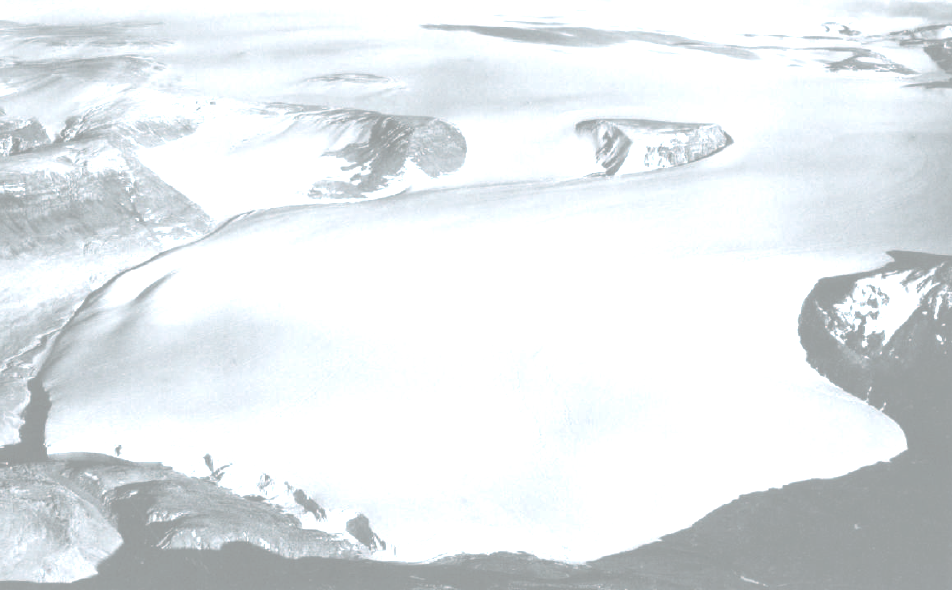
\includegraphics[width=1.5\textwidth]{figs/polaris-overexposed.png}%

\vspace{-25mm}
\hfill 
\includegraphics[width=0.17\textwidth]{figs/uafbw.png}}

\begin{document}
\graphicspath{{figs/}{../../paper/figs/}}

\maketitle


\begin{frame}[plain]

\mbox{\hspace{-9mm} 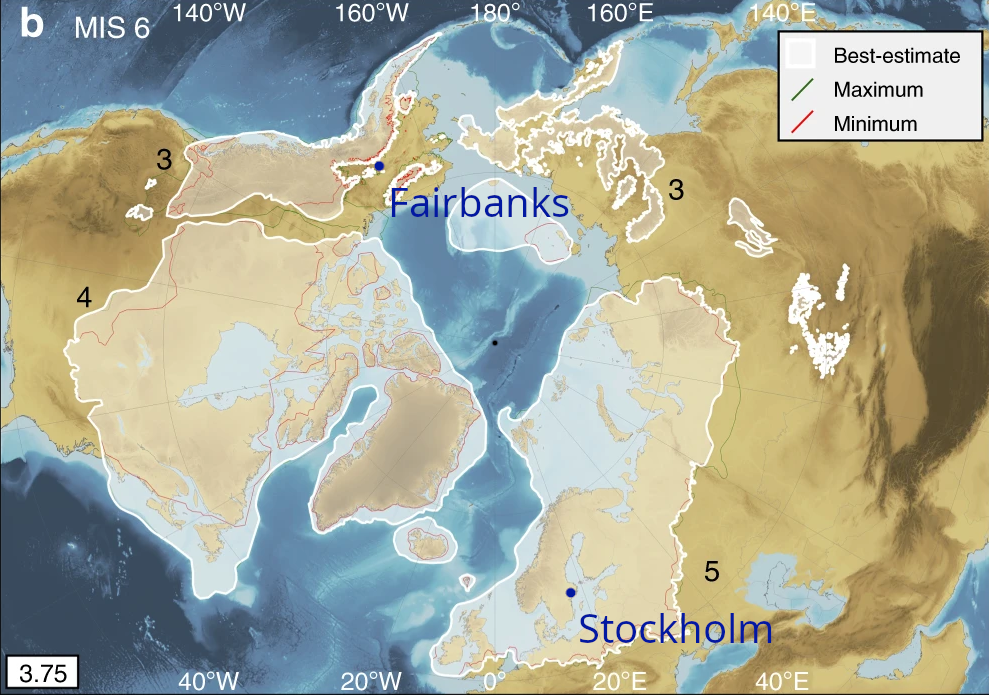
\includegraphics[width=1.15\textwidth]{nhsheets.png}}

\vspace{-2mm}
\hfill {\tiny Fig.~1 from Batchelor (2019), \emph{The configuration of Northern Hemisphere ice sheets through the Quaternary}}
\end{frame}


\begin{frame}{motivating question about glaciers and ice sheets}

\begin{itemize}
\item in a given climate and with a given topography,

\begin{center}
\aler{what is the extent of glaciation?}
\end{center}

    \begin{itemize}
    \item[$\circ$] what is the geometry, namely the surface elevation, of the ice?
    \item[$\circ$] this is a coupled climate-and-ice-flow problem
    \end{itemize}

\bigskip
\item my motivation for \aler{finite element solutions of variational inequalities} is this free-boundary problem for the surface elevation of glaciers
\end{itemize}
\end{frame}


\begin{frame}{Outline}
  \setbeamertemplate{section in toc}[sections numbered]
  \tableofcontents%[hideallsubsections]
\end{frame}

\AtBeginSection[]
{% do not put toc here this time
}

\section{variational inequalities (VIs)}

\subsection{(and coercivity)}

\begin{frame}{reminder: coercivity for gradients}

\begin{itemize}
\item let's recall a famous inequality from convex optimization
\item let $J: \RR^n \to \RR$ be a smooth objective function
\item assume the Hessian $H(x)=\grad^2 J(x)$ is uniformly symmetric positive definite (SPD), and thus $J$ is convex
\end{itemize}

\bigskip
\begin{proposition}
the gradient $F=\nabla J$ is \aler{coercive}: there exists $\alpha > 0$ so that
$$(F(x) - F(y)) \cdot (x - y) \ge \alpha \|x - y\|^2$$
\end{proposition}

\emph{proof.} By Taylor expansion, and $H \ge \alpha I$ with $\alpha=\min_{x} \lambda_{\text{min}}(H(x))$,
\begin{align*}
J(x) - J(y) &\ge F(y) \cdot (x - y) + \frac{\alpha}{2} \|x-y\|^2 \\
J(y) - J(x) &\ge F(x) \cdot (y - x) + \frac{\alpha}{2} \|y-x\|^2
\end{align*}
Add the above: \quad $0 \ge (F(y) - F(x)) \cdot (x-y) +  \alpha \|x - y\|^2$. \qed
\end{frame}


\begin{frame}{example variational inequality: classical obstacle problem}

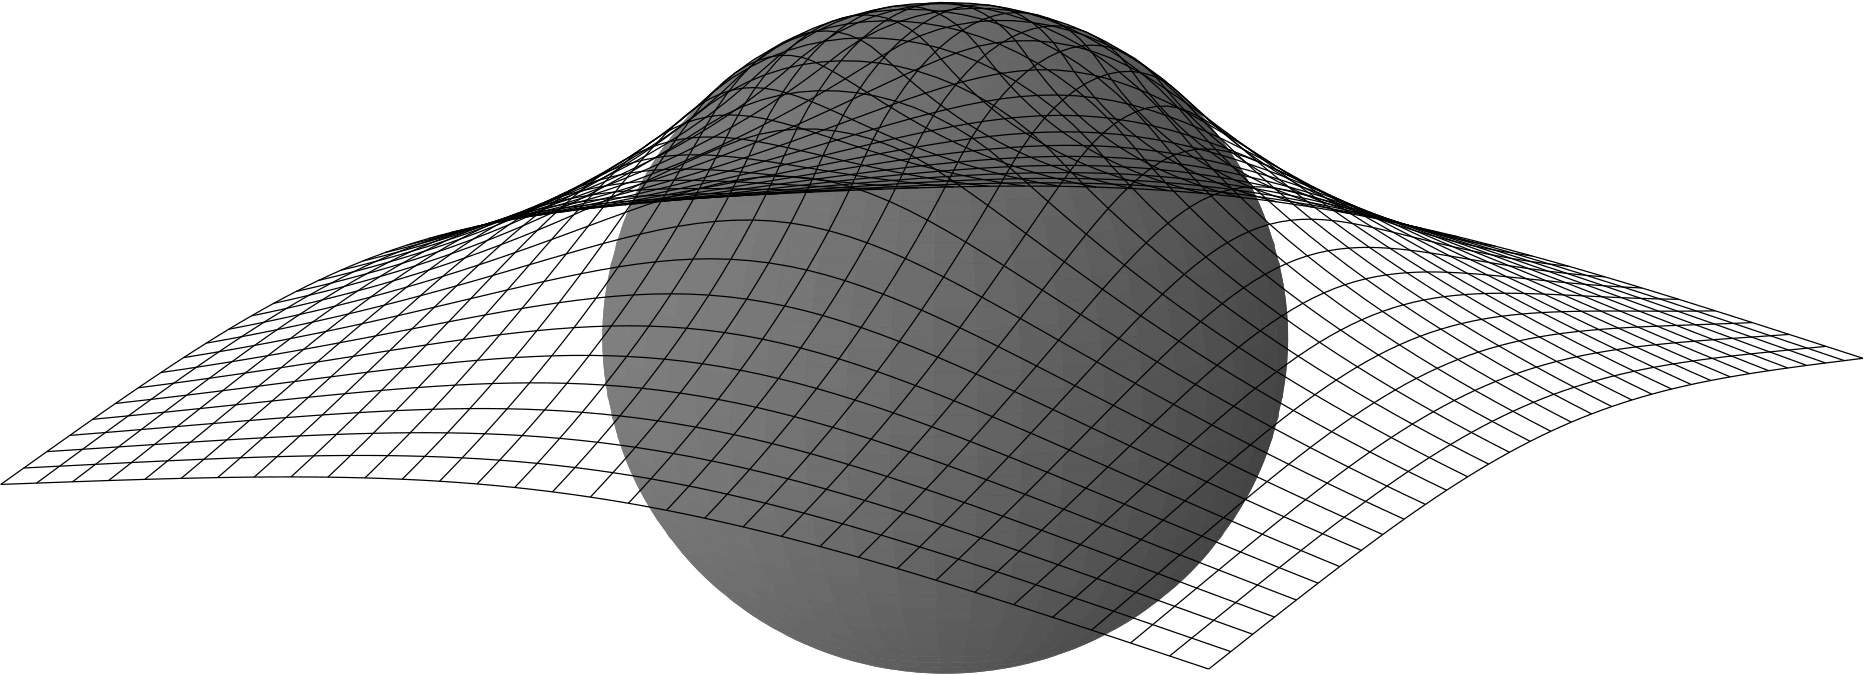
\includegraphics[width=0.55\textwidth]{figs/obstacle65.png} \qquad 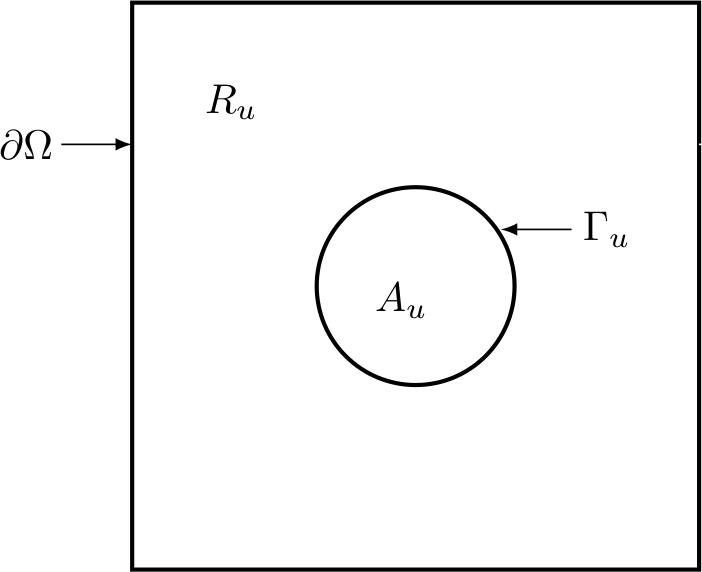
\includegraphics[width=0.35\textwidth]{figs/obstacle-sets.png}

\only<1>{
\begin{itemize}
\item given: domain $\Omega\subset \RR^2$, obstacle $\psi$, Dirichlet condition $g$, source $\varphi$
\item the \emph{admissible set}: \, $\cK = \left\{v \in H^1(\Omega) \,:\, v\big|_{\partial \Omega} = g \text{ and } v \ge \psi\right\}$
\item let $J(v) = \frac{1}{2} \int_\Omega |\grad v|^2 - \varphi v$, and consider $\min_{v\in\cK} J(v)$
\item the \emph{\aler{variational inequality}} (VI) is to find $u\in\cK$ so that
    $$\int_\Omega \grad u\cdot \grad (v-u) - \varphi (v-u) \ge 0 \quad \text{for all } v \in \cK$$

    \begin{itemize}
    \item[$\circ$] the weak form operator is $F(u)[v] = \int_\Omega \grad u\cdot \grad v - \varphi v$
    \item[$\circ$] $F$ is coercive on $H^1(\Omega)$
    \end{itemize}
\end{itemize}
}
\only<2>{
\begin{itemize}
\item the solution defines \emph{\aler{active}} $A_u = \{u = \psi\}$ and \emph{\aler{inactive}} $R_u = \{u> \psi\}$ subsets of $\Omega$, and a \emph{\aler{free boundary}} $\Gamma_u=\partial R_u \cap \Omega$
\item the intuitive/naive strong form poses the problem in terms of its solution, a kind of nonsense:
    $$-\grad^2 u = \varphi \quad \text{ on $R_u$, \qquad and \qquad} u = \psi \quad \text{ on $A_u$}$$
\end{itemize}

\vspace{20mm}
}
\end{frame}


\begin{frame}{general variational inequalities}

\begin{itemize}
\item let $\cX$ be a real, reflexive Banach space
\item let $\cK \subset \cX$ be a closed and convex subset
\item suppose $F:\cK \to \cX'$ is a continuous operator
    \begin{itemize}
    \item[$\circ$] $F$ \aler{may not} be the gradient of any objective function $J$
    \item[$\circ$] $F$ may be defined \aler{only on $\mathcal{K}$}
    \item[$\circ$] $F$ may be nonlinear
    \end{itemize}
\item suppose $\ell\in\cX'$
\item denote the general variational inequality problem as {\color{FireBrick} VI($F$,$\ell$,$\mathcal{K}$)}:
	$${\color{FireBrick} F(u)[v-u] \ge \ell[v-u] \quad \text{ for all } v \in \mathcal{K}}$$

    \begin{itemize}
    \item[$\circ$] if $\mathcal{K}$ is nontrivial, VI($F$,$\ell$,$\mathcal{K}$) is nonlinear, even when $F$ is linear
    \end{itemize}

\end{itemize}
\end{frame}


\begin{frame}{why ``$v-u$'' in the VI?}

\begin{center}
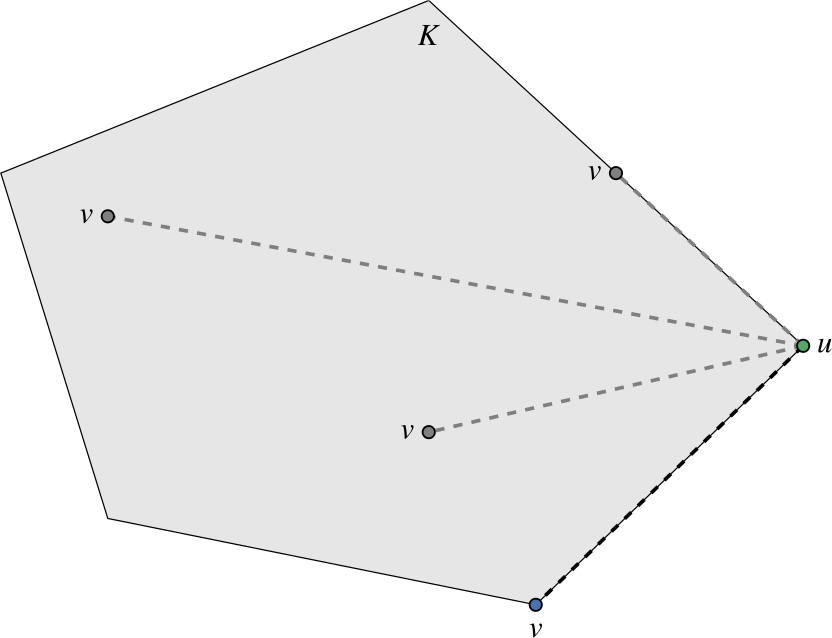
\includegraphics[width=0.7\textwidth]{figs/viconvex.png}
\end{center}

\vspace{-5mm}
\hfill {\tiny P.~Farrell figure}

\begin{itemize}
\item $v-u \in \cX$ is a vector pointing feasibly into $\cK$
\item $(F(u)-\ell)[v-u] \ge 0$ \, $\iff$ \, ``$F(u)-\ell$ is within $90^\circ$ of any $v-u$''
\end{itemize}
\end{frame}


\begin{frame}{complementarity, a key idea about VIs}

\begin{itemize}
\item if $u\in\cK$ solves the VI
$$F(u)[v-u] \ge \ell[v-u] \quad \text{ for all } v \in \mathcal{K},$$
then \aler{generally the residual $F(u)-\ell$ is nonzero}
    \begin{itemize}
    \item[$\circ$] if $\cK=\cX$ (unconstrained) then $F(u)-\ell=0$
    \end{itemize}
\item for a unilateral obstacle problem, with $\cK = \{v\in\cX\,:\,v\ge \psi\}$, the residual $F(u)-\ell$ is at least \aler{nonnegative}
    \begin{itemize}
    \item[$\circ$] the residual is a positive measure $d\mu_u = F(u)-\ell$ supported in the active set $A_u=\{x\,:\, u(x)=\psi(x)\}$
    \end{itemize}
\item for classical obstacle problem, the strong form statement of complementarity is:
	$$u\ge \psi, \quad -\grad^2 u - \varphi \ge 0, \quad (u-\psi) (-\grad^2 u - \varphi) = 0$$
\end{itemize}
\end{frame}


\begin{frame}{variational inequality $=$ constrained equation}

\begin{center}
\begin{tabular}{l|l}
\begin{minipage}[t][16mm][t]{0.4\textwidth}
unconstrained optimization:
$$\min_{u\in\mathcal{X}} J(u)$$
\end{minipage}
&
\begin{minipage}[t][16mm][t]{0.5\textwidth}
constrained optimization:
$$\min_{u\in\mathcal{K}} J(u)$$
\end{minipage}
\\ \hline
\begin{minipage}[t][16mm][t]{0.4\textwidth}
\phantom{foo}

equation for $u \in \mathcal{X}$:
$$\only<1>{F(u)=\ell}\only<2>{F(u)[v]=\ell[v] \quad \forall v \in \mathcal{X}}$$
\end{minipage}
&
\begin{minipage}[t][16mm][t]{0.5\textwidth}
\only<1>{
\phantom{foo}

\begin{center}
{\Large ?}
\end{center}
}
\only<2>{
\phantom{foo}

variational inequality for $u \in \mathcal{K}$:
$${\color{FireBrick} F(u)[v-u] \ge \ell[v-u] \quad \forall v \in \mathcal{K}}$$
}
\end{minipage}
\end{tabular}
\end{center}
\end{frame}


\begin{frame}{$\qq$-coercivity and well-posedness}

\begin{block}{continuum VI problem}
VI for $u \in \cK$:
$$F(u)[v-u] \ge \ell[v-u] \quad \forall v \in \cK$$
\end{block}

\begin{defn} $F:\cK \to \cX'$ is \aler{$\qq$-coercive} for $\qq>1$ if
  $$\left(F(v)-F(w)\right)[v-w] \ge \alpha \|v-w\|^\qq \qquad \forall v,w \in \cK$$
\end{defn}

\begin{thm}[well-posedness; Kinderlehrer \& Stampaccia (1980)] 
if $F$ is $\qq$-coercive and continuous then the continuum VI problem is well-posed
\end{thm}
\end{frame}


\AtBeginSection[] {
    \begin{frame}{Outline}
    \setbeamertemplate{section in toc}[sections numbered]
    \tableofcontents[currentsection]%,hideallsubsections]
    \end{frame}
}

\section{a new \emph{a priori} error bound for finite element methods on VIs}


\begin{frame}{finite element (FE) approximation of the VI}

\begin{cproblem}
VI for $u \in \cK$:
$$F(u)[v-u] \ge \ell[v-u] \quad \forall v \in \cK$$
\end{cproblem}

\begin{feproblem}
VI for $u_h \in \cK_h$:
$$F_h(u_h)[v_h-u_h] \ge \ell[v_h-u_h] \quad \forall v_h \in \cK_h$$
\end{feproblem}

conforming assumptions\only<1>{:}\only<2-3>{\aler{?}}
\begin{itemize}
\item $\cK_h \subset \cX_h \subset \cX$

\only<1>{\vspace{22mm}}
\item<2-3> \aler{generally $F_h\neq F$}

\only<2>{\vspace{22mm}}
\item<3> \aler{generally $\cK_h \not\subseteq \cK$}
\end{itemize}

\vspace{-25mm}
\hfill \only<3>{\begin{tikzpicture}[scale=1.1, domain=0.0:4.0, samples=200]
  \draw[black,thin,->] (-0.3,0.0) -- (4.5,0.0) node [xshift=2mm] {$x$};
  \draw plot (\x, {1.5 + 0.8 * cos(1.8*\x r)});
  \node[yshift=-2mm] at (2.0, 0.7) {$b$};
  \newcommand{\xlist}{0.0, 1.0, 1.4, 2.4, 3.0, 4.0}
  \foreach \x [remember=\x as \lastx] in \xlist {
      \draw (\x, 0.0) circle (1.5pt);
      \filldraw (\x, {1.5 + 0.8 * cos(1.8*\x r)}) circle (1.5pt);
      \draw[dashed] (\lastx, {1.5 + 0.8 * cos(1.8*\lastx r)}) -- (\x, {1.5 + 0.8 * cos(1.8*\x r)});
  }
  \node[yshift=3mm] at (3.0, 0.0) {$x_i$};
  \node[xshift=3mm, yshift=-7mm] at (0.0, 2.3) {$b_h$};
\end{tikzpicture}
}
\end{frame}


\begin{frame}{\emph{a priori} error bound}

\begin{thm}[B~'24] assume $F$ is $\qq$-coercive with $\qq>1$ and $\alpha>0$, and Lipschitz continuous.  then there is $c=c(\|u\|,\|u_h\|,\alpha)>0$ so that
\begin{align*}
\|u-u_h\|^\qq &\le \frac{2}{\alpha} \left[\inf_{v\in\aler{\cK}} \left(F(u)-\ell\right)[v-u_h] + \inf_{v_h\in\aler{\cK_h}} \left(F(u)-\ell\right)[v_h-u]\right] \\
   &\quad\, + \frac{2}{\alpha} \left(F(u_h)-F_h(u_h)\right)[u_h] + c \inf_{v_h\in\aler{\cK_h}} \|v_h - u\|^{\qq'}
\end{align*}
\end{thm}

\begin{itemize}
\only<1>{\item in the unconstrained case ($\cK=\cX$ and $\cK_h=\cX_h$), with no variational crimes ($F_h=F$), this is \aler{Cea's lemma} in a Banach space:
    $$\|u-u_h\|^\qq \le c \inf_{v_h\in\cX_h} \|v_h - u\|^{\qq'}$$

\vspace{5.5mm}
\phantom{foo}}
\only<2>{\item if $\cX$ is a Hilbert space, $F(u)[v]=(Au,v)$ is linear, $\cX \subset \cH$ for some Hilbert space $\cH$, $\qq=2$, and with no variational crimes ($F_h=F$), then this is \aler{Falk's (1974) theorem} for VIs:
{\small
\begin{align*}
\|u-u_h\|^2 &\le \frac{2}{\alpha} \|Au-\ell\|_{\cH'} \left(\inf_{v\in\cK} \|v-u_h\|_{\cH} + \inf_{v_h\in\cK_h} \|v_h-u\|_{\cH}\right) \\
   &\quad\, + c \inf_{v_h\in\cK_h} \|v_h - u\|^2
\end{align*}
}}
\only<3>{\item for unilateral \aler{obstacle problems} $\cK = \{v\ge \psi\}$, with $d\mu_u=F(u)-\ell$ a positive measure supported in the active set $A_u$, this says
\begin{align*}
\|u-u_h\|^\qq &\le \frac{2}{\alpha} \left(\inf_{v\in\cK} \int_{A_u} v-u_h\,d\mu_u + \inf_{v_h\in\cK_h} \int_{A_u} v_h-u \,d\mu_u\right) \\
   &\quad\, + \frac{2}{\alpha} \left(F(u_h)-F_h(u_h)\right)[u_h] + c \inf_{v_h\in\cK_h} \|v_h - u\|^{\qq'}
\end{align*}
}
\end{itemize}
\end{frame}


\section{the standard glacier model}

\begin{frame}{the free-boundary problem for glacier surface elevation}

\hfill 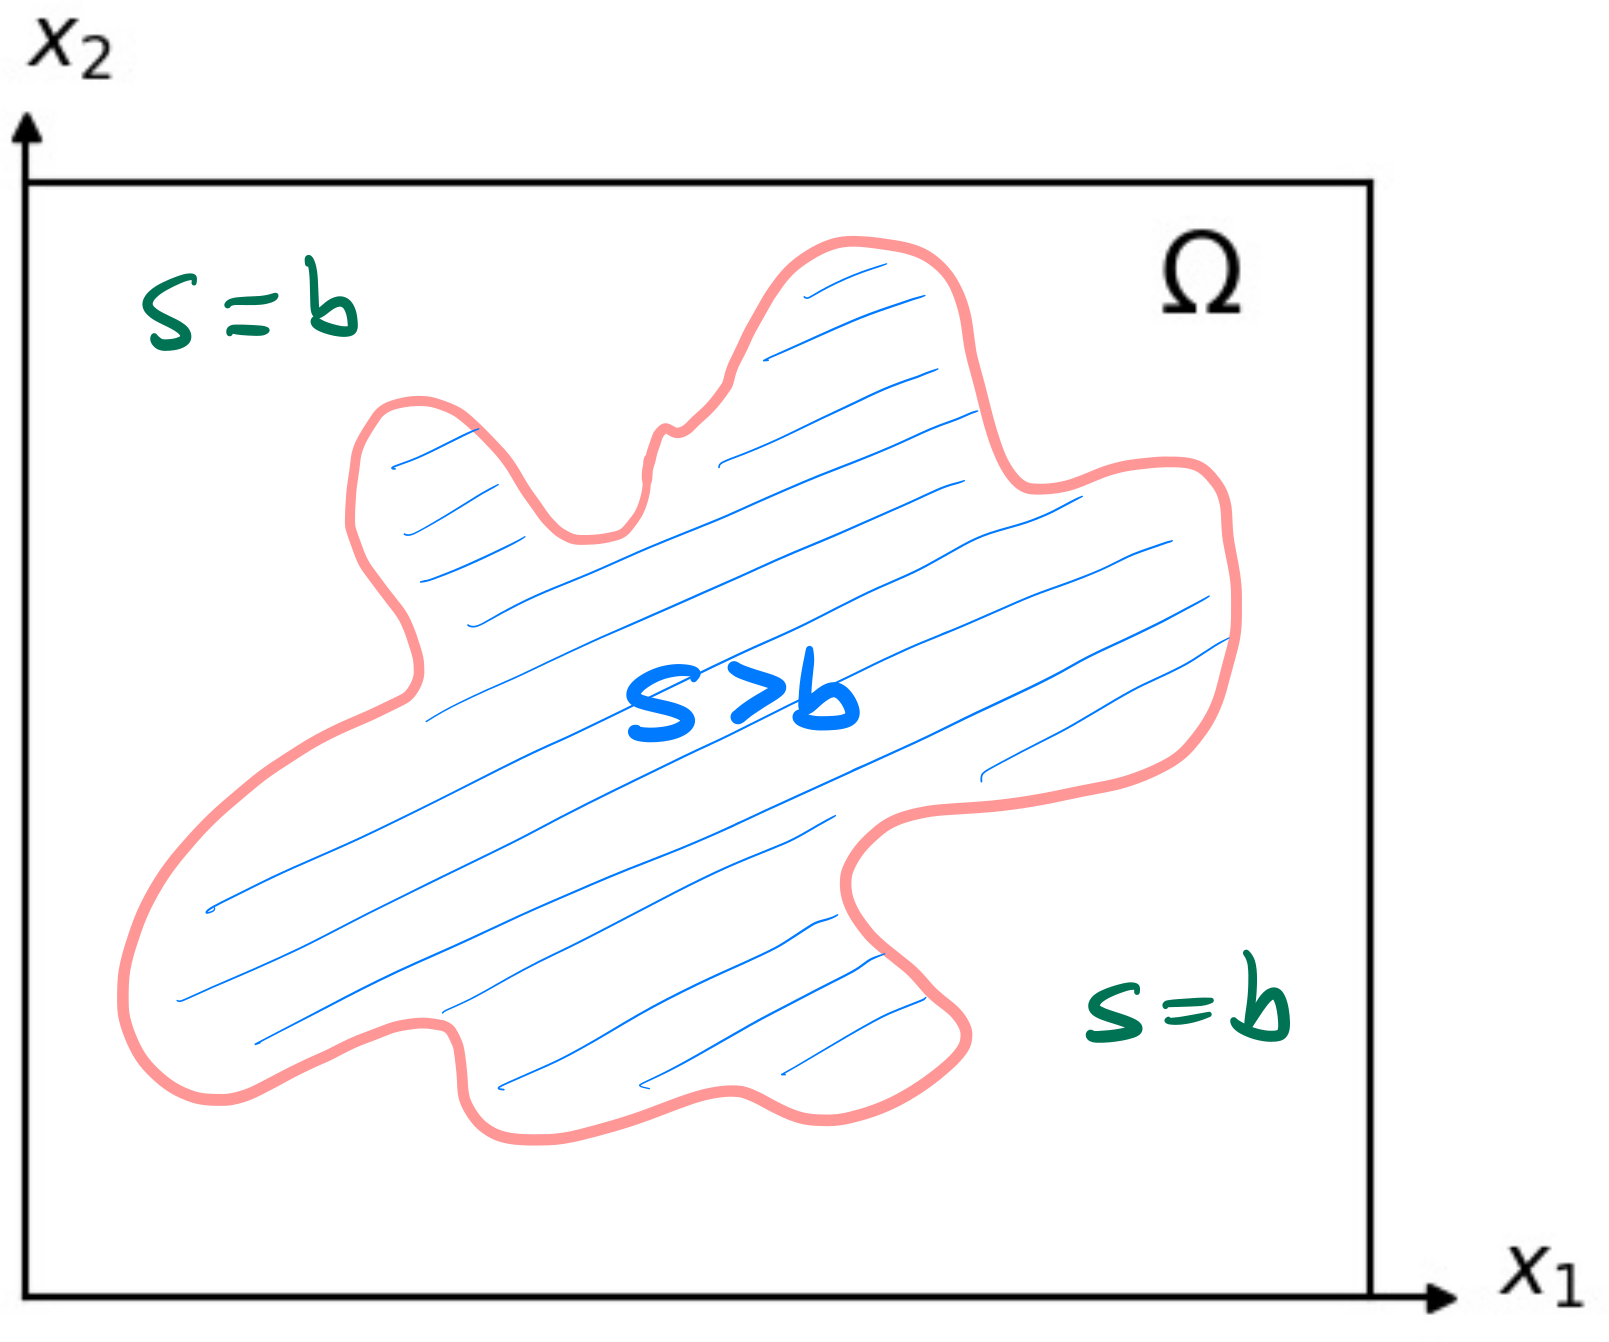
\includegraphics[width=0.4\textwidth]{mapplane}

\vspace{-39mm}

\begin{minipage}[t]{60mm}
{\small
\begin{itemize}
\item $\Omega \subset \RR^2$ fixed domain
\item $a(t,x)$ surface mass balance data
\item $b(x)$ bed elevation data
\item \aler{$s(t,x)$ surface elevation (solution)}
\item $\bn_s = (- \grad s,1)$ surface-normal vector
\item $\bu|_s(t,x)$ surface value of ice velocity, extended by zero to bare land
\end{itemize}
}
\end{minipage}

\begin{itemize}
\item an obstacle problem, in strong form, holds in $[0,T] \times \Omega$:
\begin{align*}
s - b &\ge 0 &&\phantom{x} \\
\frac{\partial s}{\partial t} - \bu|_s \cdot \bn_s - a &\ge 0 \\
(s - b) \left(\frac{\partial s}{\partial t} - \bu|_s \cdot \bn_s - a\right) &= 0
\end{align*}
\end{itemize}
\end{frame}


\begin{frame}{the free-boundary problem for glacier surface elevation}

\begin{itemize}
\item free surface equation:
   $$\frac{\partial s}{\partial t} - \bu|_s \cdot \bn_s - a = 0$$
\item the complementarity problem is the \aler{true free-boundary meaning of the free surface equation}:
\begin{align*}
s - b &\ge 0 &&\phantom{x} \\
\frac{\partial s}{\partial t} - \bu|_s \cdot \bn_s - a &\ge 0 \\
(s - b) \left(\frac{\partial s}{\partial t} - \bu|_s \cdot \bn_s - a\right) &= 0
\end{align*}

    \begin{itemize}
    \item[$\circ$] this applies regardless of dynamical model within the ice
    \item[$\circ$] the free surface equation holds where there is ice
    \item[$\circ$] $a\le 0$ where there is no ice
    \end{itemize}
\item this free-boundary problem appears first in (Calvo et al 2003), but only for shallow ice
\end{itemize}
\end{frame}


\begin{frame}{Glen-Stokes equations within the ice}

\hfill 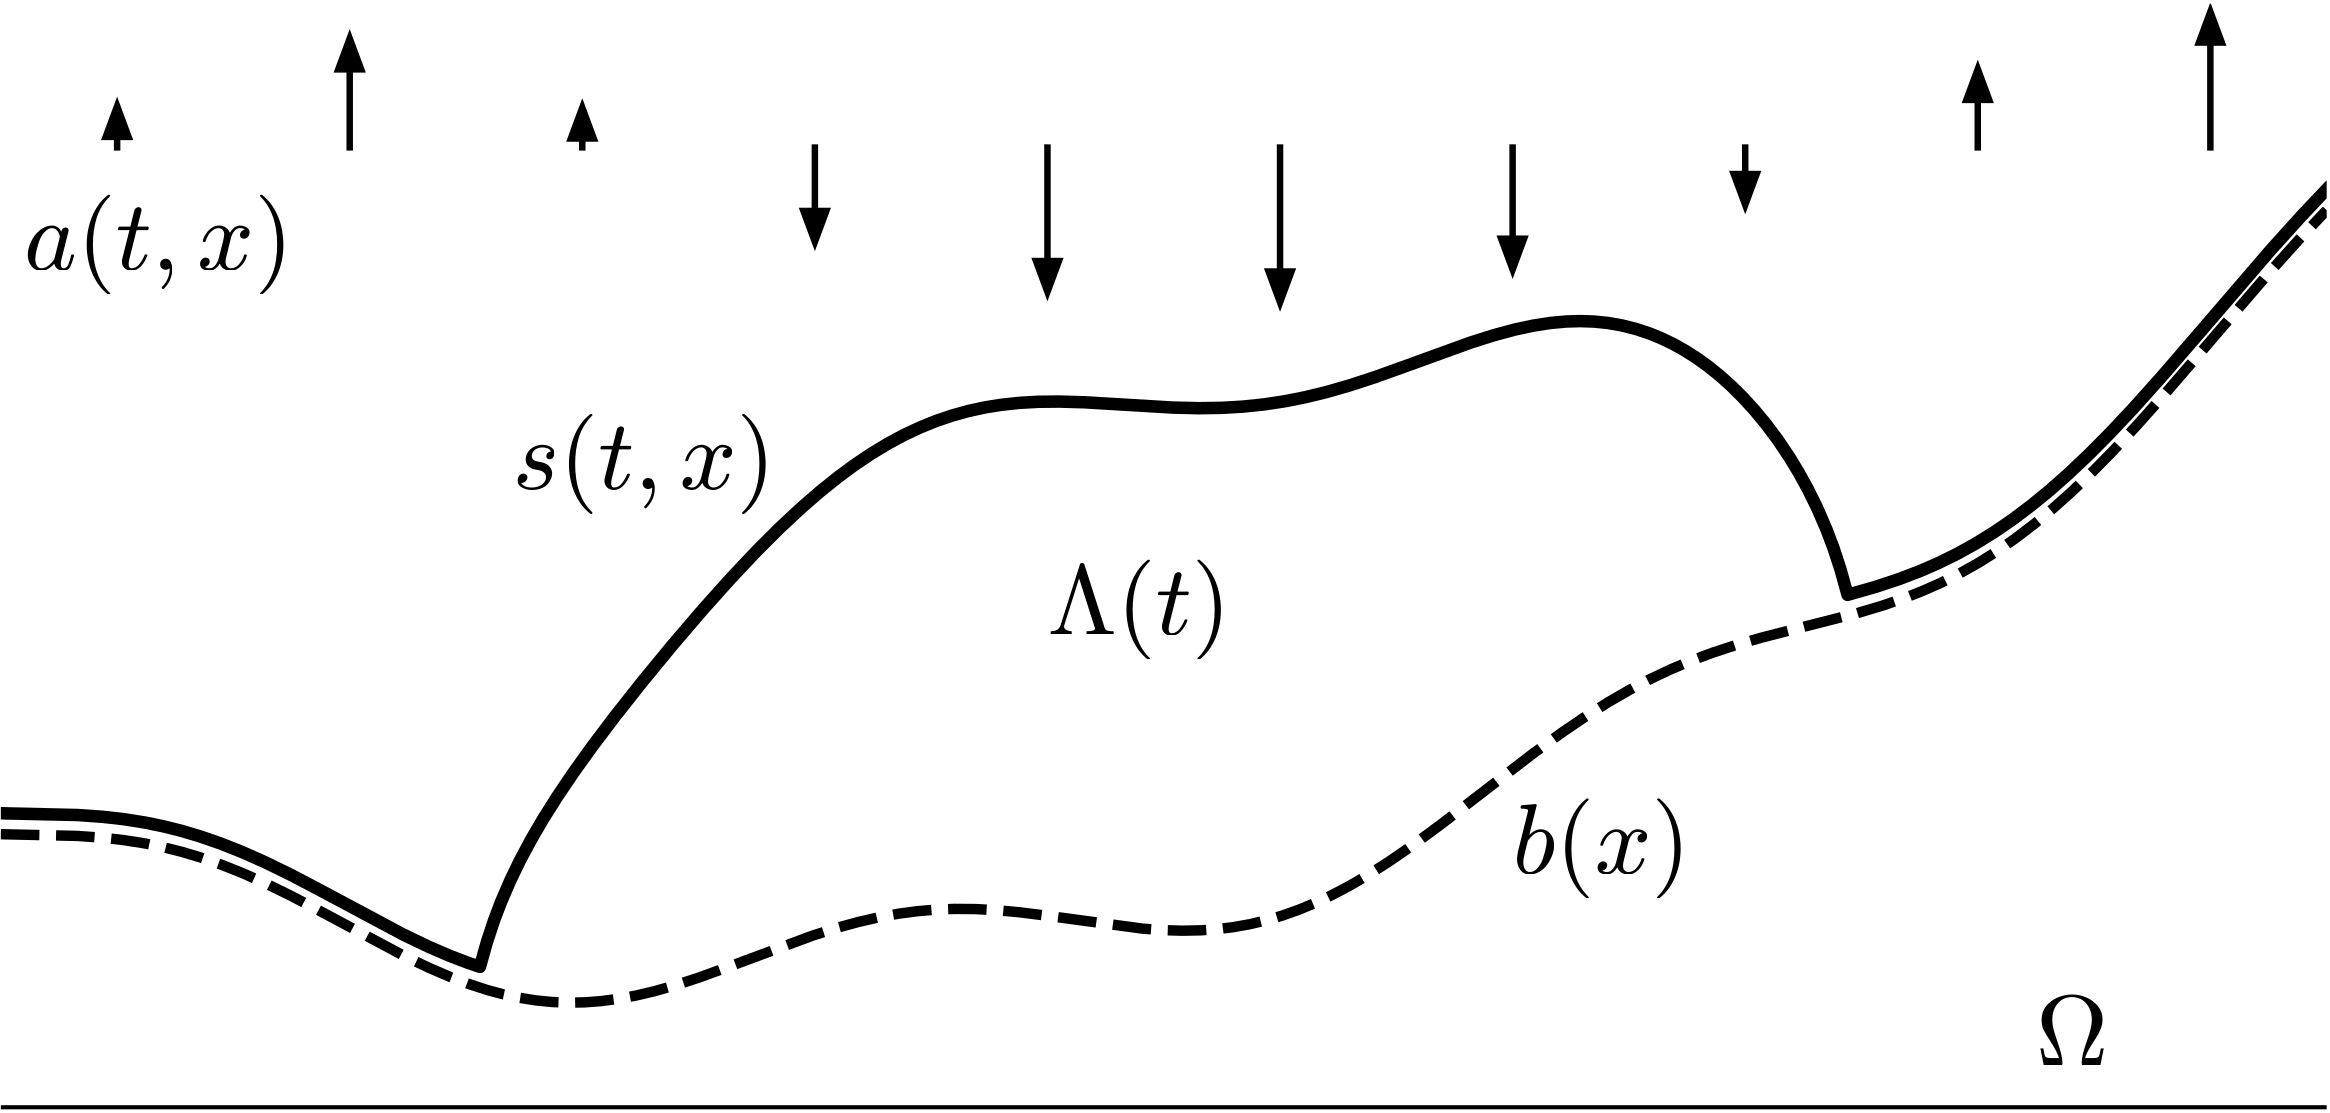
\includegraphics[width=0.45\textwidth]{stokesdomain.png}

\begin{itemize}
\item define \aler{${\displaystyle \Lambda(t) = \{(x,z)\,:\,b(x)<z<s(t,x)\}}$}
\item Glen-Stokes equations in $\Lambda(t)$ with $\pp = (\nn + 1)/\nn \approx 4/3$:
\begin{align*}
- \nabla \cdot \left(2 \nu(D\bu)\, D\bu\right) + \nabla p &= \rhoi \bg  \\
\nabla \cdot \bu &= 0
\end{align*}
where $D\bu = \frac{1}{2}\left(\grad\bu + \grad\bu^\top\right)$ is the strain-rate tensor

and $\nu(D\bu) = \nu_0 |D\bu|^{\pp-2}$ is the viscosity
\item stress boundary conditions:
\begin{align*}
&\left(2 \nu(D\bu) D\bu - pI\right) \bn_s = \bzero   && \where{on $\Gamma_s \subset \partial\Lambda(t)$} \\
&\beta(\bu,D\bu)=0 && \where{on $\Gamma_b \subset \partial\Lambda(t)$}
\end{align*}
\end{itemize}
\end{frame}


\newcommand{\stdblock}{
\begin{align*}
s - b &\ge 0 & &\where{in $\Omega$} \\
\frac{\partial s}{\partial t} - \bu|_s \cdot \bn_s - a &\ge 0 \\
(s - b) \left(\frac{\partial s}{\partial t} - \bu|_s \cdot \bn_s - a\right) &= 0 \\
- \nabla \cdot \left(2 \nu_0 |D\bu|^{\pp-2}\, D\bu\right) + \nabla p &= \rhoi \bg && \where{in $\Lambda(t)$} \\
\nabla \cdot \bu &= 0 \\
\left(2 \nu_0 |D\bu|^{\pp-2} D\bu - pI\right) \bn_s &= \bzero && \where{on $\Gamma_s \subset \partial\Lambda(t)$} \\
\beta(\bu,D\bu) &= 0 && \where{on $\Gamma_b \subset \partial\Lambda(t)$}
\end{align*}
}

\begin{frame}{\underline{the} standard model for glacier evolution?}

\stdblock

\bigskip
\newtheorem*{smodel}{standard model}

\begin{smodel}
a complementarity problem (obstacle problem) in $[0,T]\times \Omega$, over a fixed $\Omega \subset \RR^2$, \aler{coupled} to a Glen-Stokes problem for $\bu$ and $p$, within the $s$-dependent ice domain $\Lambda(t) \subset \RR^3$; the solution is a triple $(s,\bu,p)$
\end{smodel}
\end{frame}


\begin{frame}{mathematical knowledge about the standard model}

\begin{itemize}
\item \dots is limited, for now, to the \aler{fixed-domain Stokes problem}

\begin{thm}[Jouvet \& Rappaz, 2011]
over a fixed $C^1$ domain $\Lambda\subset\RR^3$, the $\pp>1$ Stokes problem
\begin{align*}
- \nabla \cdot \left(2 \nu_0 |D\bu|^{\pp-2}\, D\bu\right) + \nabla p &= \rhoi \bg && \where{in $\Lambda$} \\
\nabla \cdot \bu &= 0 \\
\left(2 \nu_0 |D\bu|^{\pp-2} D\bu - pI\right) \bn_h &= \bzero && \where{on $\Gamma_s\subset\partial\Lambda$} \\
\beta(\bu,D\bu) &= 0 && \where{on $\Gamma_b\subset\partial\Lambda$}
\end{align*}
is well-posed for the solution $(\bu,p) \in W^{1,\pp}(\Omega;\RR^3) \times L^{\pp'}(\Omega)$
\end{thm}

\item thus, at each instant $t$, if the surface elevation $s$ is known and smooth, then the velocity $\bu$ and pressure $p$ are uniquely-determined
\end{itemize}
\end{frame}


\begin{frame}{the standard model wants implicit time-stepping}

{\footnotesize
\stdblock
}

\bigskip
\begin{block}{standard model (as a dynamical system)}
the model is an inequality-constrained \aler{differential algebraic equation} (DAE) system in $\infty$ dimensions
\end{block}

\begin{itemize}
\item \aler{implicit} methods are the usual recommendation for the infinitely-stiff limit of ODE systems, namely DAEs
\end{itemize}
\end{frame}



\section{are implicit steps of the standard model well-posed?}

\begin{frame}{a single implicit time step of the standard model}

\begin{itemize}
\item let $\Delta t>0$ and denote \aler{$s \approx s(t_k)$} and $s^{k-1}\approx s(t_{k-1})$
\item change notation: \aler{$\Lambda(s) = \{(x,z)\,:\,b(x) < z < s(x)\}$}
\item consider a \aler{backward Euler time step} of the non-sliding model:
{\small
\begin{align*}
s - b &\ge 0 & &\where{in $\Omega$} \\
s - \Delta t\, \bu|_s \cdot \bn_s - \ell &\ge 0 \\
(s - b) \left(s - \Delta t\, \bu|_s \cdot \bn_s - \ell\right) &= 0 \\
- \nabla \cdot \left(2 \nu_0 |D\bu|^{\pp-2}\, D\bu\right) + \nabla p &= \rhoi \bg && \where{in $\Lambda(s)$} \\
\nabla \cdot \bu &= 0 \\
\left(2 \nu_0 |D\bu|^{\pp-2} D\bu - pI\right) \bn_s &= \bzero && \where{on $\Gamma_s \subset \partial\Lambda(s)$} \\
\bu &= 0 && \where{on $\Gamma_b \subset \partial\Lambda(s)$}
\end{align*}
}
\item with source term
{\small
    $$\ell(x) = s^{k-1}(x) + \Delta t\,\int_{t_{k-1}}^{t_k} a(t,x)\,dt$$
}
\item the solution, if it exists, is a triple $(s,\bu,p)$ for the new time $t_k$
\end{itemize}
\end{frame}


\subsection{(core issue: is the surface motion $\qq$-coercive?)}

\begin{frame}{the surface motion term}

\begin{itemize}
\item regarding the questions of well-posedness and surface elevation errors, we focus on the key term

\begin{defn}
the \aler{surface motion} in the standard model: \, $\Phi(s) = -\bu_s\cdot \bn_s$
\end{defn}

\item \dots and on the key question
\begin{question}
is the surface motion $\Phi(s)$ $\qq$-coercive?

are there $\qq>1$ and $\alpha>0$ so that
$$(\Phi(s) - \Phi(\sigma))[s-\sigma] \stackrel{?}{\ge} \alpha \|s-\sigma\|_{\cX}^\qq$$
for all $s,\sigma \in \cK = \{\omega \in \cX\,:\, \omega\big|_{\partial \Omega} = b\big|_{\partial \Omega} \, \text{ and } \, \omega \ge b\}$, where $\cX$ is a Banach space to be determined?
\end{question}
\end{itemize}
\end{frame}


\begin{frame}{is the surface motion coercive?}

\begin{question}
$$(\Phi(s) - \Phi(\sigma))[s-\sigma] \stackrel{?}{\ge} \alpha \|s-\sigma\|_{\cX}^\qq$$
\end{question}

\begin{itemize}
\item the answer is \aler{no} for general bumpy beds
\item for surfaces $s_1,s_2\in\cK$ below we compute
\begin{align*}
\Phi(s_1) &= 0 \\
\Phi(s_2) &= 0 \\
\|s_1-s_2\|_{\cX} &> 0
\end{align*}

\hfill 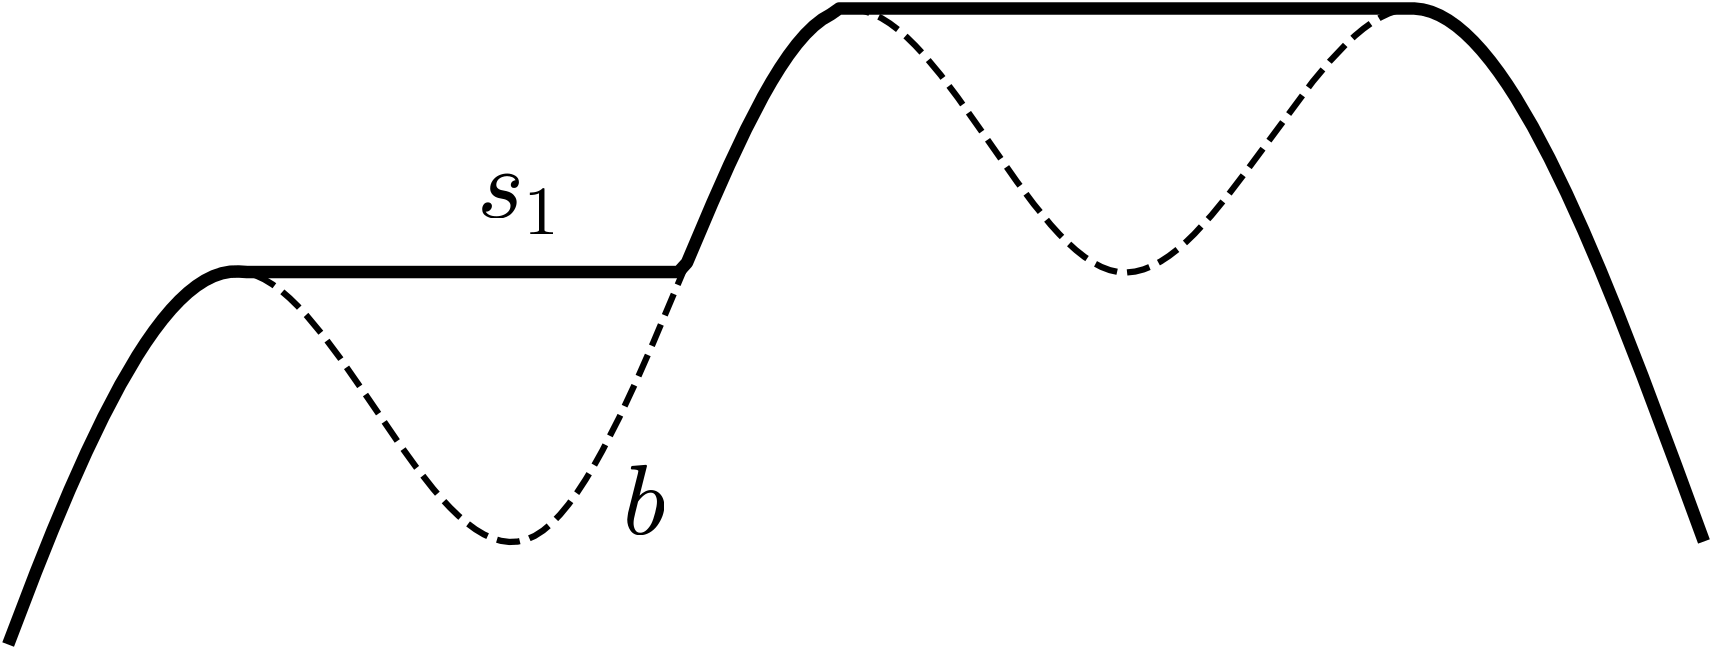
\includegraphics[width=0.35\textwidth]{figs/filled.png} \qquad 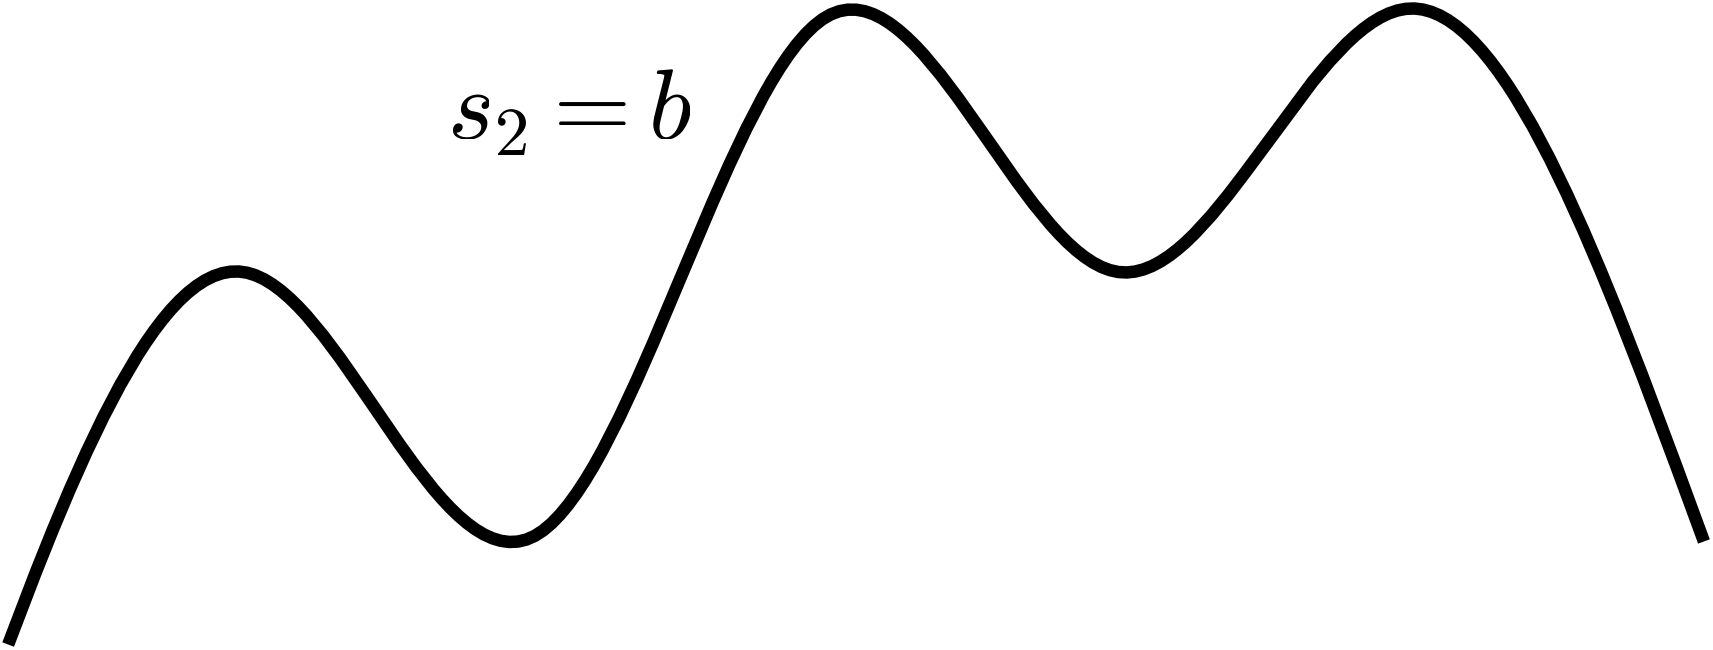
\includegraphics[width=0.35\textwidth]{figs/icefree.png}
\item neither surface generates flow when we solve Stokes over $\Lambda(s_i)$
    \begin{itemize}
    \item[$\circ$] note $\Lambda(s_2)=\emptyset$
    \end{itemize}
\end{itemize}
\end{frame}


\begin{frame}{is the \underline{regularized} surface motion coercive?}

\begin{question}
$$(\Phi^{\aler{\eps}}(s) - \Phi^{\aler{\eps}}(\sigma))[s-\sigma] \stackrel{?}{\ge} \alpha^{\aler{\eps}} \|s-\sigma\|_{\cX}^\qq$$
\end{question}

\begin{itemize}
\only<1>{
\item for $\eps>0$ small and $H_0$ comparable to ice thickness, define
   $$\Phi^\eps(s) = (u|_s,v|_s) \cdot \grad s - (1-\eps) w|_s - \eps \Div\left(\Gamma H_0^5 |\grad s|^2\grad s\right)$$
\item this \aler{regularization of the surface value of the vertical velocity}, using the shallow ice approximation formula, breaks the symmetry on the last slide
    \begin{itemize}
    \item[$\circ$] it prefers flat ice surfaces
    \end{itemize}
\item $\eps=0$ case returns $\Phi(s)$:
   $$\Phi^0(s) = (u|_s,v|_s) \cdot \grad s - w|_s = -\bu_s\cdot \bn_s$$
}
\only<2>{
\item a \aler{numerical experiment}, computing these ratios for $\eps=0.1$ and $H_0=1000$ m,
$$\frac{(\Phi^{\aler{\eps}}(s_1) - \Phi^{\aler{\eps}}(s_1))[s_1-s_2]}{\|s_1-s_2\|_{\cX}^4}$$
\aler{gives evidence of $\qq=4$-coercivity}
\item randomly chosen pairs $s_1,s_2 \in W^{1,4}(\Omega)$ from $10^3$ states which were generated using FSSA acceleration (L\"ofgren et al.~2022)

\bigskip
\centering
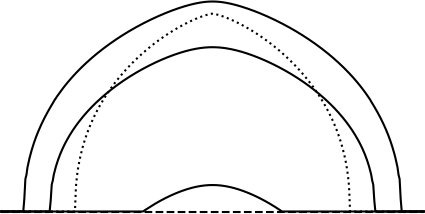
\includegraphics[width=0.35\textwidth]{figs/snapsflat.png} \qquad 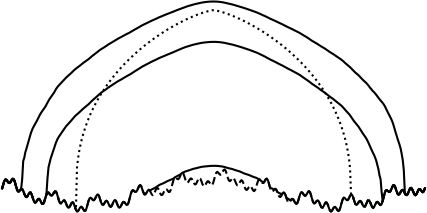
\includegraphics[width=0.35\textwidth]{figs/snapsrough.png}
}
\only<3>{
\item ratios without regularization:

\medskip
\hfill
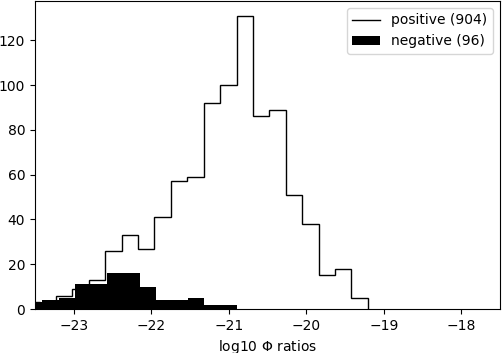
\includegraphics[width=0.32\textwidth]{figs/bflat500mNOREG.png} \qquad 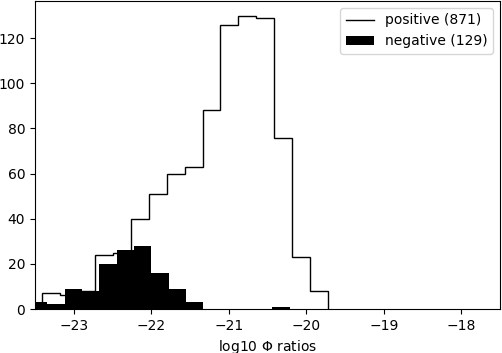
\includegraphics[width=0.32\textwidth]{figs/brough500mNOREG.png}

\item \aler{ratios with regularization}:

\medskip
\hfill
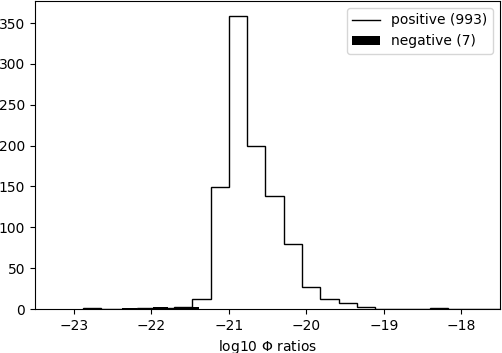
\includegraphics[width=0.32\textwidth]{figs/bflat500mREG.png} \qquad 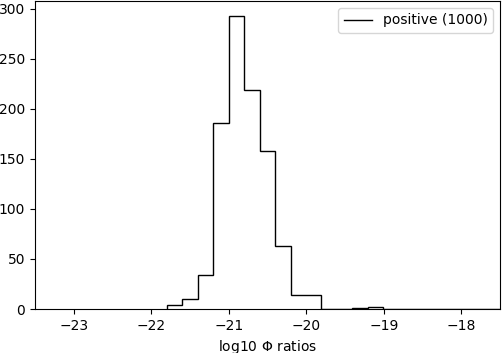
\includegraphics[width=0.32\textwidth]{figs/brough500mREG.png}
}
\only<4>{
\item mesh refinement ($\Delta x=2$ km, 1 km, 500 m) eliminates negative ratios:

\medskip
\hfill
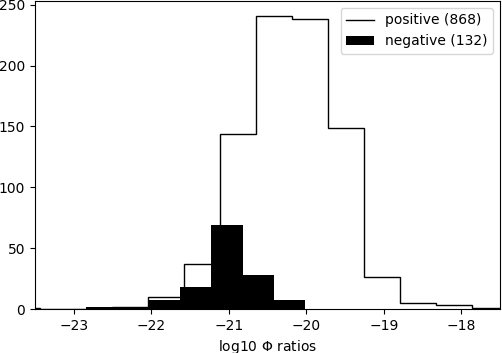
\includegraphics[width=0.27\textwidth]{figs/brough2000mREG.png}
\quad 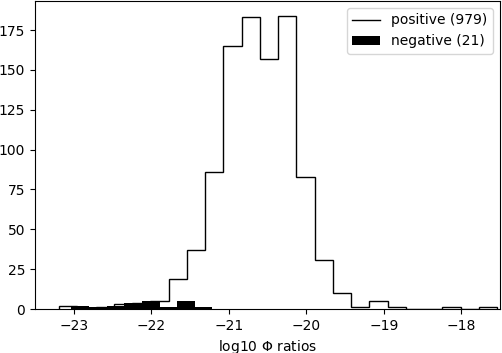
\includegraphics[width=0.27\textwidth]{figs/brough1000mREG.png}
\quad 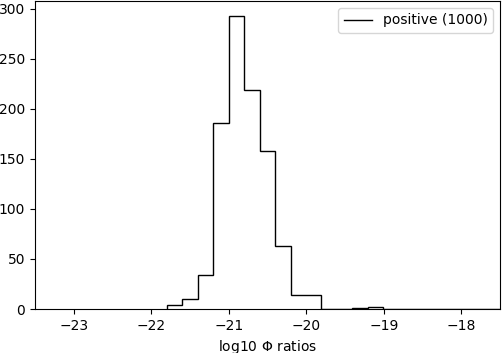
\includegraphics[width=0.27\textwidth]{figs/brough500mREG.png}

\item perhaps $\alpha_\eps \sim 10^{-21} \,\text{m}^{9/4}\,\text{s}^{-1}$?

\vspace{19mm}
}
\end{itemize}
\end{frame}


\begin{frame}{an implicit time step of the regularized standard model}

\begin{itemize}
\item define
    $$F^\eps(\sigma)[\omega] = \int_\Omega \left(\sigma + \Delta t\,\Phi^\eps(\sigma)\right) \omega$$
\end{itemize}

\begin{defn}
the weak form \aler{backward Euler time-step problem} is to find the surface elevation $s \approx s(t_k,x)$ in $\cK =\{\sigma\,:\, \sigma \ge b \text{ and } \sigma|_{\partial\Omega} = b_{\partial\Omega}\} \subset \cX$, where $\cX = W^{1,4}(\Omega)$, solving the VI
$$F^\eps(s)[\sigma-s] \ge \ell[\sigma-s] \quad \text{for all } \sigma \in \cK$$
\end{defn}
\end{frame}


\begin{frame}{well-posedness is only conjectural}

\begin{conjecture}[B~'24]
$\Phi^\eps$ is $4$-coercive,

so the backward Euler time-step problem is well-posed for $s$
\end{conjecture}

\smallskip
\begin{itemize}
\item this is a license to go hunting for a numerical solution to the glaciation problem
\end{itemize}

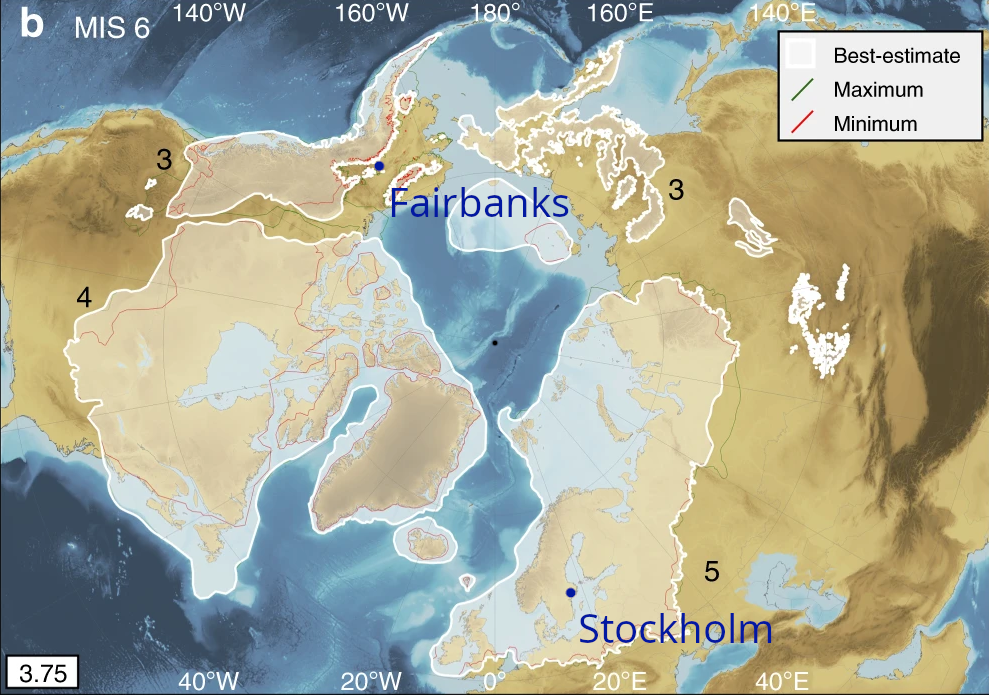
\includegraphics[width=0.45\textwidth]{nhsheets} \hfill 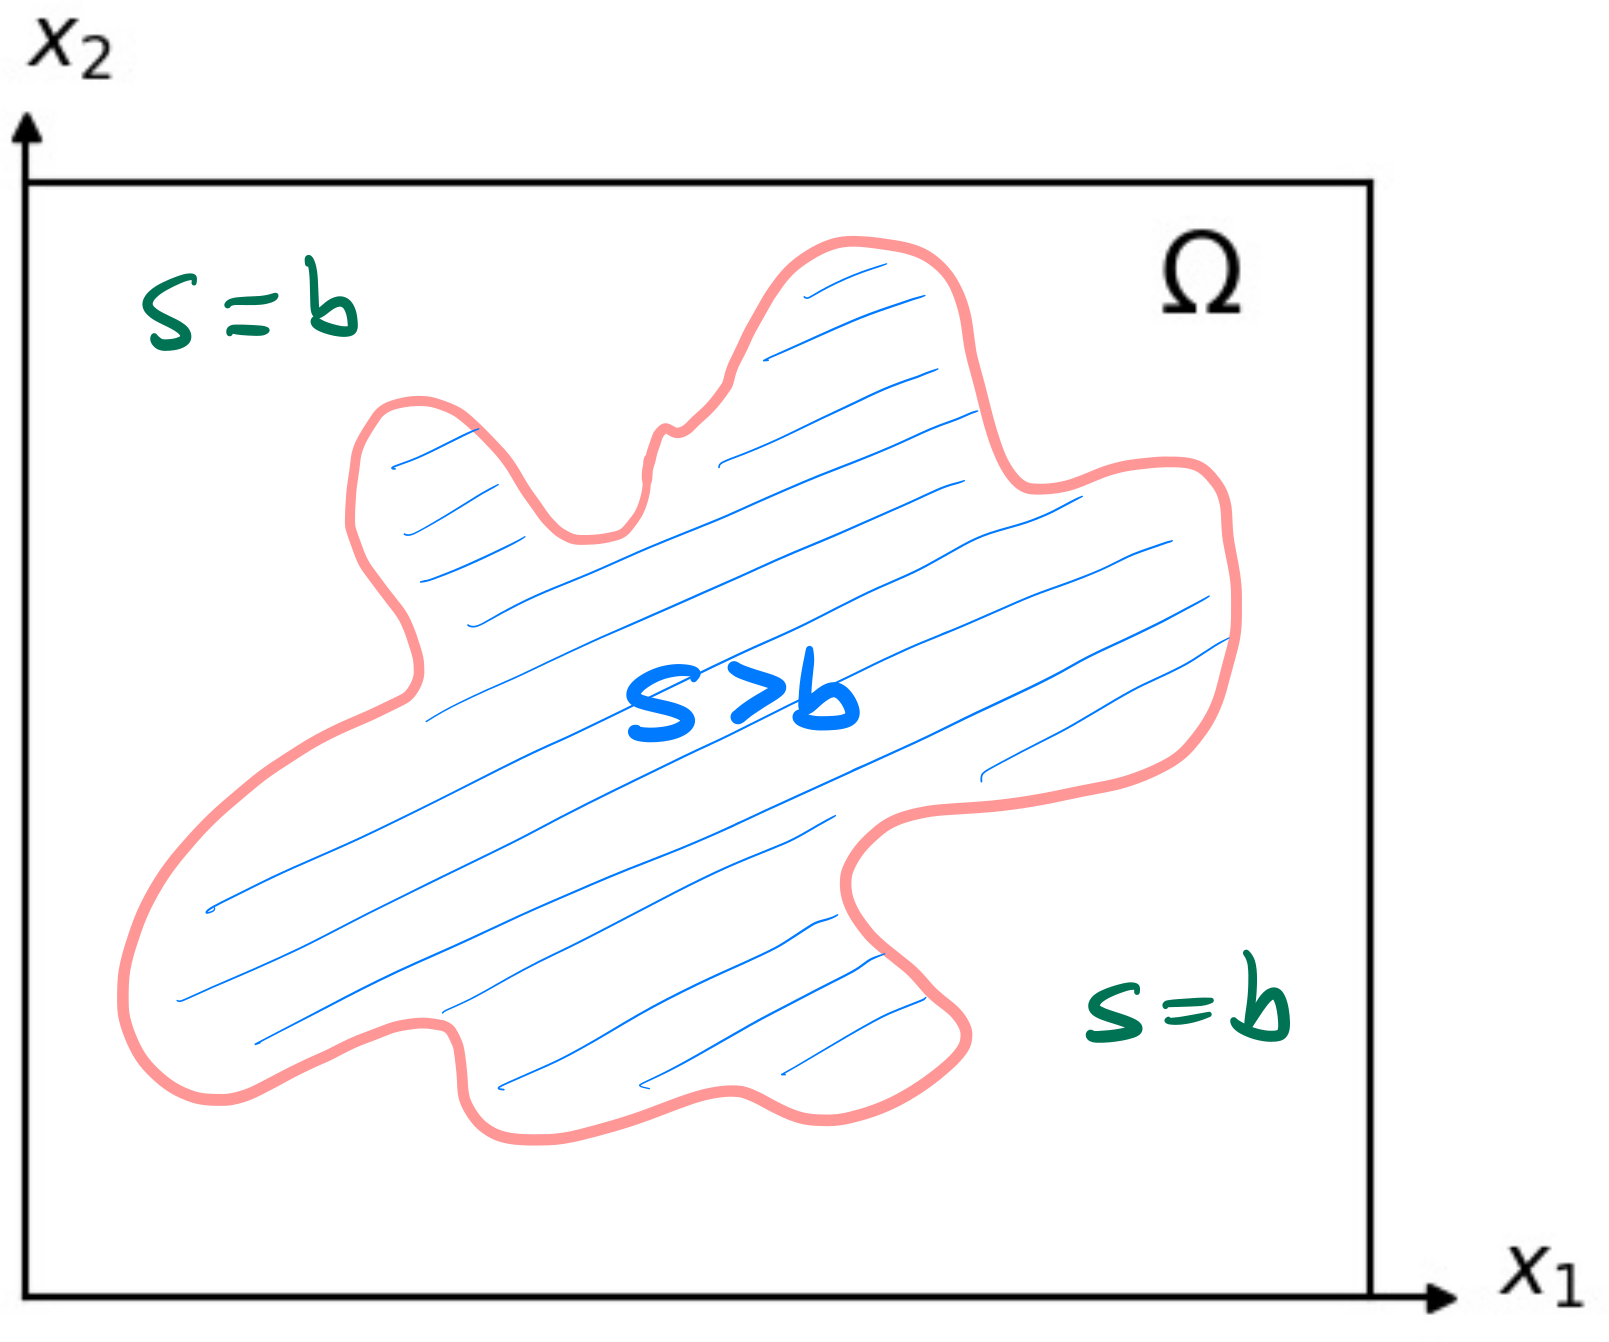
\includegraphics[width=0.4\textwidth]{mapplane}
\end{frame}


\section{application:  \emph{a priori} bound on surface elevation errors}

\begin{frame}{FE method}

\begin{center}
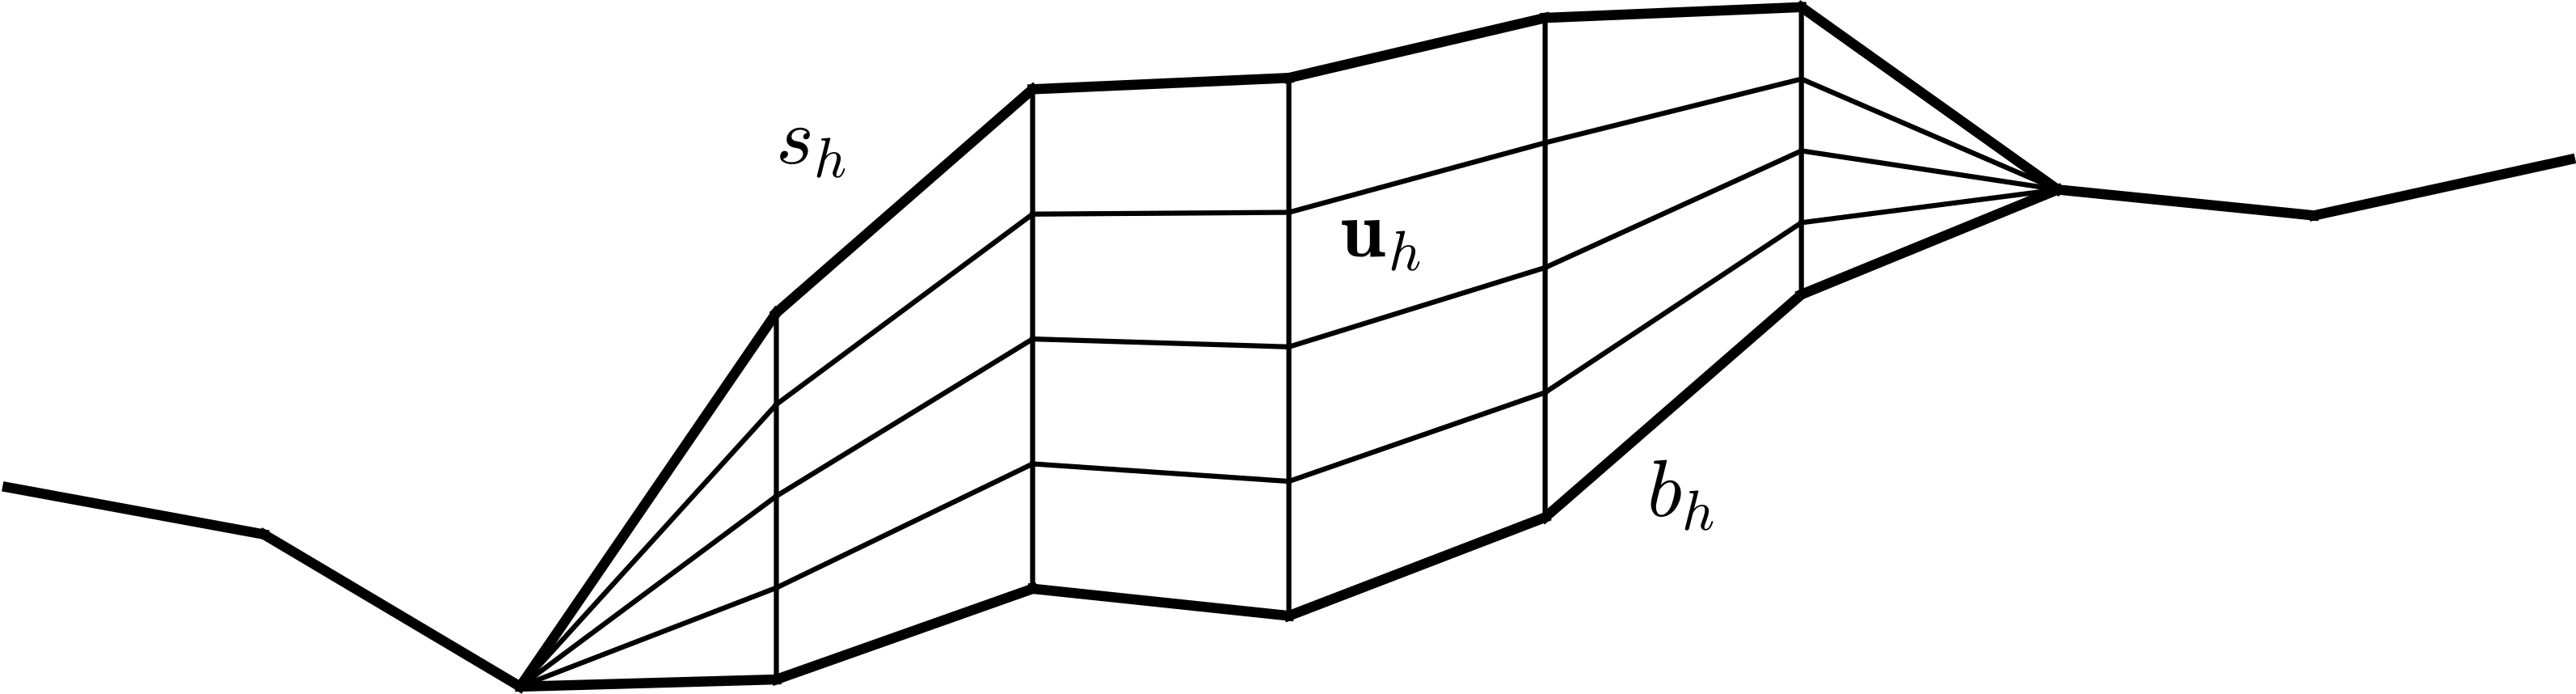
\includegraphics[width=0.8\textwidth]{extruded}
\end{center}

\begin{itemize}
\item proposed, simplest FE spaces:
   \begin{itemize}
   \item[$\circ$] an extruded mesh
   \item[$\circ$] $b_h,s_h \in P_1$ in 2D, over $\Omega$
   \item[$\circ$] $\bu_h,p_h \in P_2 \times P_1$ in 3D, over $\Lambda(s_h)$
   \end{itemize}
\item discrete admissible set: $\cK_h = \{\sigma_h \,:\, \sigma_h \ge b_h \text{ and } {\sigma_h}|_{\partial\Omega} = {b_h}|_{\partial\Omega}\}$
\item FE method for $s_h\in\cK_h$:
   $$F_h(s_h)[\sigma_h-s_h] \ge \ell[\sigma_h-s_h] \quad \text{for all } \sigma_h \in \cK_h$$
\end{itemize}

\phantom{x}
\end{frame}


\newcommand{\result}{
\begin{align*}
\|s_h-s\|_{\cX}^4 &\le \, \frac{c_0}{\Delta t} \int_{\Omega_A(s)} (b - \ell) (b_h - b) \\
   &\quad\, + c_1(s_h) \big\|\bu_h - \bu\big\|_{W^{1,4/3}(\Lambda(s_h))} \\
   &\quad\, + c_2 \|\Pi_h(s) - s\|_{\cX}^{4/3}
\end{align*}
}

\begin{frame}{bound on surface elevation errors for implicit step}

\noindent 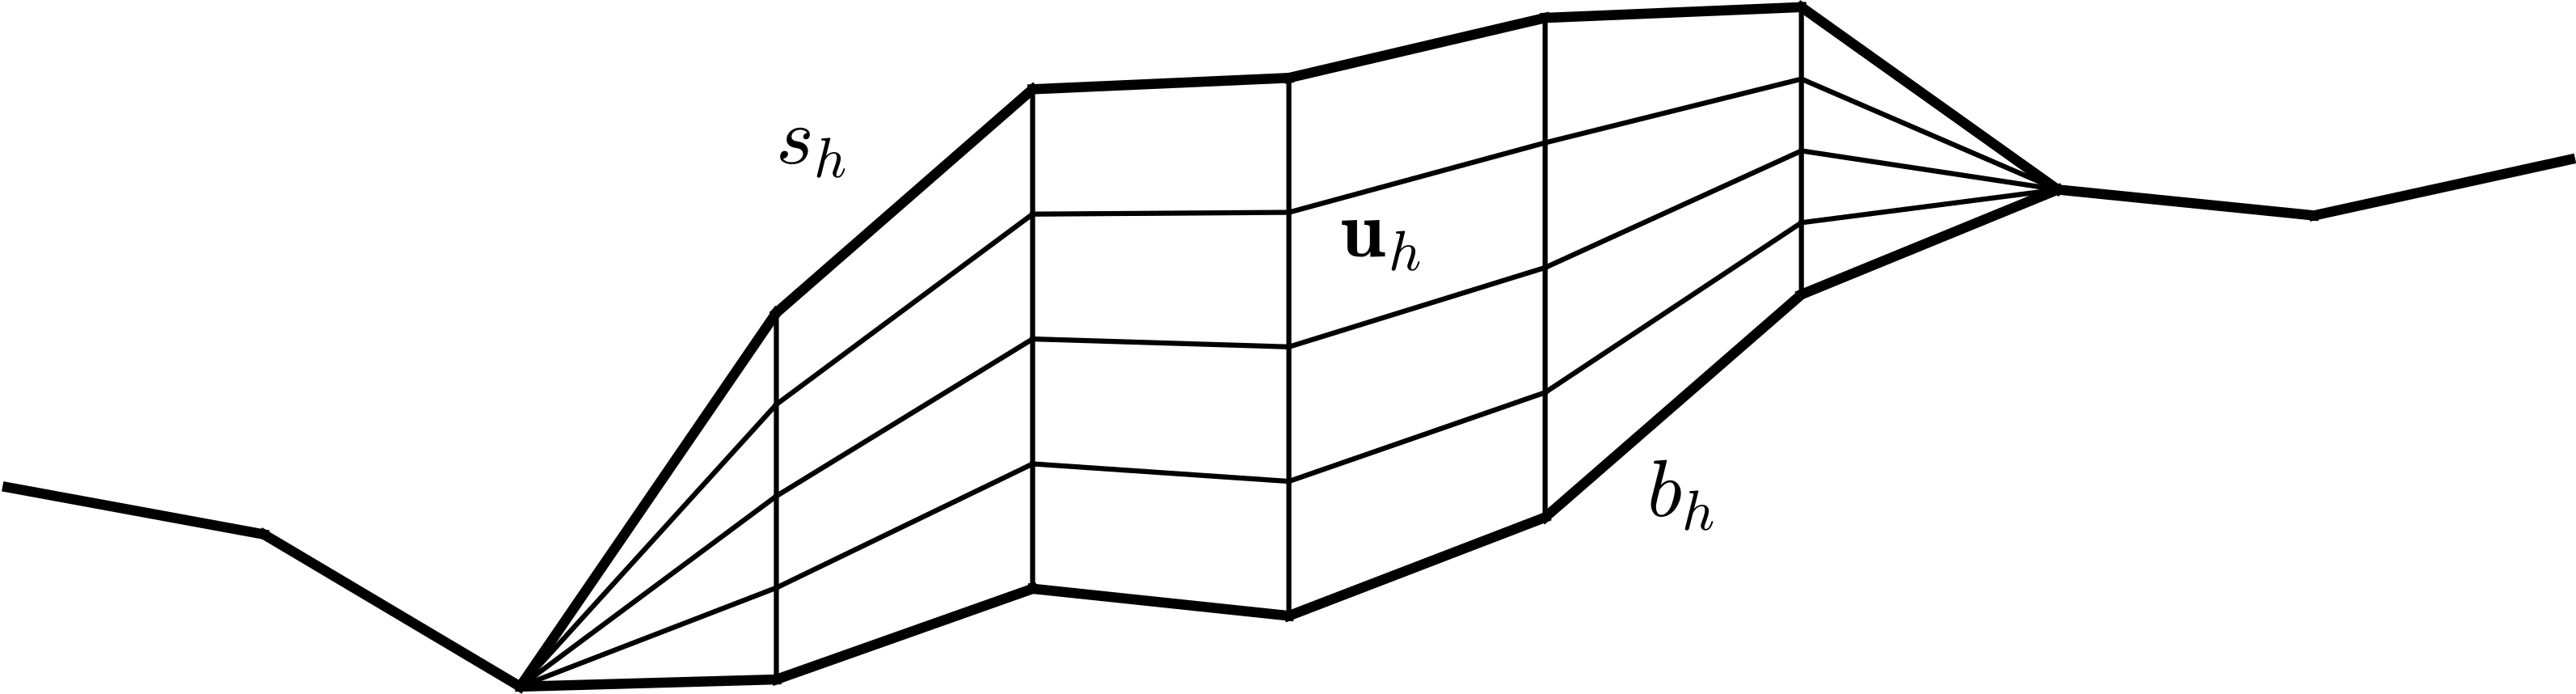
\includegraphics[width=0.6\textwidth]{extruded} \hfill 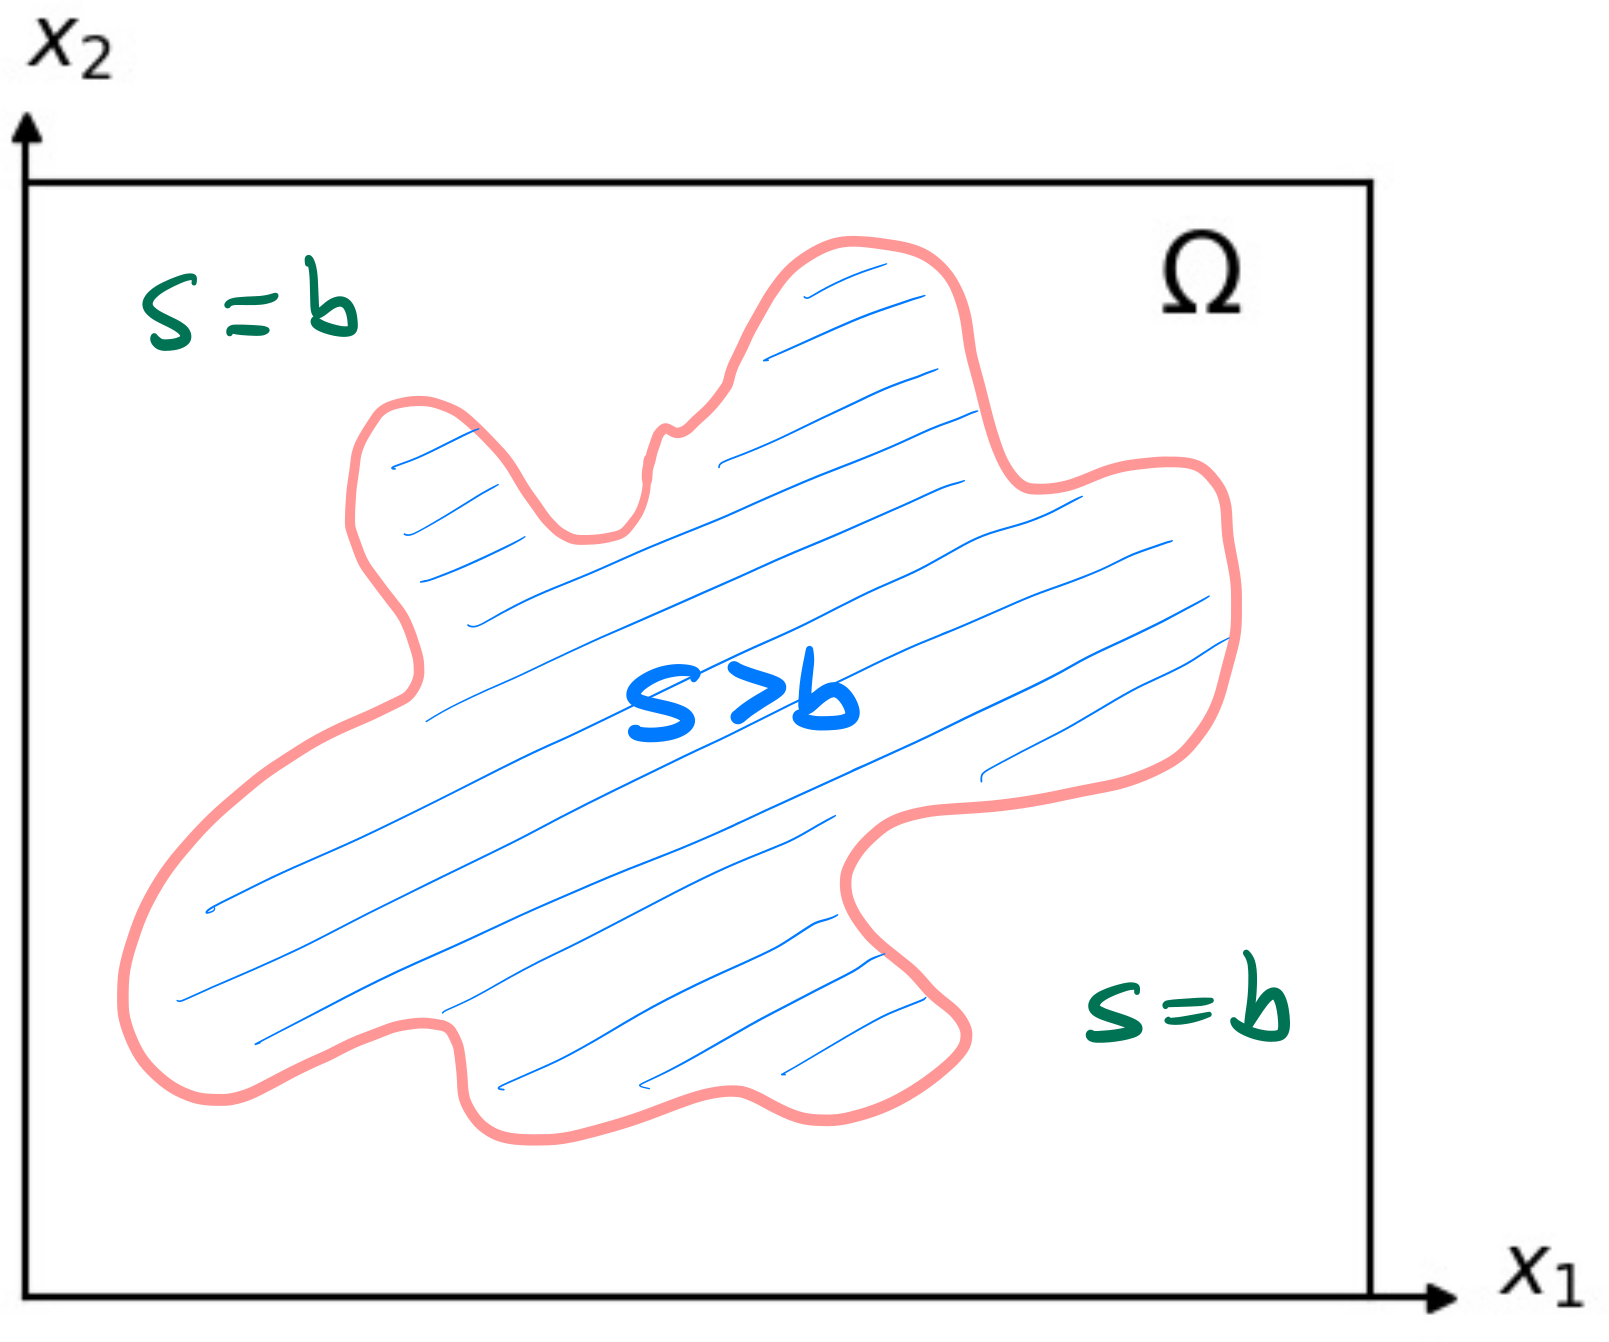
\includegraphics[width=0.23\textwidth]{mapplane}

\medskip
\begin{thm}[B'24]
Suppose $\Phi^\eps$ is $4$-coercive in $\cX = W^{1,4}(\Omega)$.  In discretizing the bed, ensure that $b_h\ge b$.  Let $\Omega_A(s)$ be the exact active set, the ice-free area.  Let $\Pi_h$ be interpolation and truncation $\cK \to \cK_h$.  Then the error in the FE surface elevation $s_h\in\cK_h$ is bounded by 3 terms:
\result
\end{thm}
\end{frame}


\begin{frame}{bound on surface elevation errors for implicit step}

\begin{thm}[B'24]
\result
\end{thm}

\noindent \emph{Proof.} Apply the general \emph{a priori} theorem.  Of the four terms, the ``$\inf_{v\in \cK}$'' term can be replaced by zero because $\cK_h\subset \cK$ from the bed construction.  Estimate the ``$\inf_{v_h\in\cK_h}$'' term for the residual by considering the residual measure; it simplifies to $d\mu_u=b-\ell$ in $\Omega_A(s)$.  Estimate the ``$(F(u_h)-F_h(u_h))[u_h]$'' term by bounding the surface trace of the Stokes velocity solution.  Estimate the Cea's lemma term in the usual interpolation way, but remember to truncate into $\cK_h$. \qed
\end{frame}


\begin{frame}{summary}
\begin{itemize}
\item implicit time-stepping for variational inequalities is needed for the standard geometry-evolving Stokes model for glaciers
    \begin{itemize}
    \item[$\circ$] both a differential-algebraic system and a free-boundary problem
    \end{itemize}
\item<2-4> \textbf{conjecture.} an SIA-regularized form of the surface motion $\Phi(s) = -\bu|_s\cdot \bn_s$, with $\bu|_s$ from the Glen-Stokes problem, is $4$-coercive over admissible $s\in W^{1,4}(\Omega)$
    \begin{itemize}
    \item[$\circ$] implies that each continuous-space, backward Euler time step problem is well-posed
    \end{itemize}
\item<3-4> \textbf{theorem.} for abstract $\qq$-coercive operators, the FE approximation of the VI problem has an \emph{a priori} bound with 4 terms \dots
\item<4> \textbf{theorem.} supposing the conjecture, the FE surface elevation error, in a backward Euler step of the standard glacier model is bounded by a sum of terms:
    \begin{enumerate}
    \item error in discretizing the bed elevation ($b_h$ versus $b$)
    \item error in numerically solving the Stokes equations ($\bu_h$ versus $\bu$)
    \item a Cea's lemma term for the surface elevation ($s_h$ versus $\Pi_h(s)$) \strut
    \end{enumerate}
\end{itemize}
\end{frame}


\begin{frame}{references}

{\footnotesize % inputed at end of slides.tex

\newcommand{\sdoi}[1]{\,{\scriptsize \href{https://doi.org/#1}{doi:#1}}}
\newcommand{\surl}[2]{\,{\scriptsize \href{#1}{#2}}}

\begin{itemize}
%\item E.~Bueler (2021). \emph{Conservation laws for free-boundary fluid layers}, SIAM J.~Appl.~Math.~81 (5), 2007--2032 \sdoi{10.1137/20M135217X}
%\item E.~Bueler (2022). \emph{Performance analysis of high-resolution ice-sheet simulations}, J.~Glaciol.~69 (276), 930--935 \sdoi{10.1017/jog.2022.113}
%\item E.~Bueler \& P.~Farrell (2024).  \emph{A full approximation scheme multilevel method for nonlinear variational inequalities}, SIAM J.~Sci.~Comput.~46 (4), \sdoi{10.1137/23M1594200}
\item E.~Bueler (2024). \emph{Surface elevation errors in finite element {S}tokes models for glacier evolution}, submitted \surl{https://arxiv.org/abs/2408.06470}{arxiv:2408.06470}
\item N.~Calvo and others (2003). \emph{On a doubly nonlinear parabolic obstacle problem modelling ice sheet dynamics}, SIAM J.~Appl.~Math.~63 (2), 683--707 \sdoi{10.1137/S0036139901385345}
%\item T.~Isaac, G.~Stadler, \& O.~Ghattas (2015). \emph{Solution of nonlinear Stokes equations \dots ice sheet dynamics}, SIAM J.~Sci.~Comput., 37 (6), B804--B833 \sdoi{10.1137/140974407}
%\item G.~Jouvet \& E.~Bueler (2012). \emph{Steady, shallow ice sheets as obstacle problems: well-posedness and finite element approximation}, SIAM J.~Appl.~Math.~72 (4), 1292--1314 \sdoi{10.1137/110856654}
\item G.~Jouvet \& J.~Rappaz (2011). \emph{Analysis and finite element approximation of a nonlinear stationary {S}tokes problem \dots}, Adv.~Numer.~Analysis 2011 (164581) \sdoi{10.1155/2011/164581}
%\item A.~L{\"o}fgren, J.~Ahlkrona \& C. Helanow (2022). \emph{Increasing stable time-step sizes of the free-surface problem arising in ice-sheet simulations},~J. Comput. Phys.: X 16 (100114) \sdoi={10.1016/j.jcpx.2022.100114}
\end{itemize}
}
\end{frame}

\end{document}
